
\section{Pretraining Hyperparameters} 

We detail our pretraining hyperparameter values in Table \ref{tab:pretrain_hyperparams} below.

\begin{table}[h]
\centering
\begin{tabular}{p{2cm} p{1.5cm} p{0.7cm} p{1.2cm} p{0.6cm} p{0.6cm} p{0.6cm} p{1cm} p{1.4cm} p{0.8cm} }\\

\toprule
Model & Optimizer & LR & beta & eps & WD & MB & Warmup & Final LR & MLM \\
\midrule
BERT-Base & Decoupled AdamW & 5e-4 & [0.9,0.98] & 1e-6 & 1e-5 & 512 & 6\% & 0.02LR & 0.15 \\
MosaicBERT-Base & Decoupled AdamW & 5e-4 & [0.9,0.98] & 1e-6 & 1e-5 & 512 & 6\% & 0.02LR  & 0.3 \\
BERT-Large & Decoupled AdamW & 2e-4 & [0.9,0.98] & 1e-6 & 1e-5 & 256 & 6\% & 0.02LR  & 0.15 \\
MosaicBERT-Large & Decoupled AdamW & 2e-4 & [0.9,0.98] & 1e-6 & 1e-5 & 256 & 6\% & 0.02LR & 0.3 \\
\bottomrule

\end{tabular}

\caption{Pretraining hyperparameters for BERT-Base, MosaicBERT-Base, BERT-Large and MosaicBERT-Large. LR = learning rate, WD = weight decay, MB = Microbatch and MLM = Masked Language Modeling ratio. All pretraining runs were done on $8\times$ A100-80 GB GPUs.}
\label{tab:pretrain_hyperparams}
\end{table}

All pretraining runs followed a warmup + linear decay learning rate schedule. Evaluation was done every 2000 batches, and checkpoints were saved every 3500 batches - both of which slow down training slightly.




\section{Finetuning Hyperparameters}

We used the hyperparameters in Table \ref{tab:finetuning_hyperparameters} for finetuning all BERT and MosaicBERT models.
All finetuning datasets used a maximum sequence length of 256 tokens. 
We found that these values worked well across all tasks for BERT-Base, MosaicBERT-Base, and MosaicBERT-Large; BERT-Large however was somewhat less performant on QQP for some pretraining seeds.


\begin{table}[h!]
\begin{tabular}{p{1.5cm} p{2cm} p{2.0cm} p{1.5cm} p{2.cm} p{1.0cm} p{1.0cm} }
\toprule
Task & learning rate & beta & epsilon & weight decay & epochs & seeds \\ \hline
MNLI & 5e-5 & [0.9, 0.98] & 1e-6 & 5e-6 & 3 & 1 \\
QNLI & 1e-5 & [0.9, 0.98] & 1e-6 & 1e-6 & 10 & 1 \\
QQP & 3e-5,1.5e-5 & [0.9,0.988] & 1e-6 & 3e-6 & 5 & 1\\
RTE & 1e-5 & [0.9, 0.98] & 1e-6 & 1e-5 & 3 & 5\\
CoLA & 5e-5 & [0.9, 0.98] & 1e-6 & 5e-6 & 10 & 4 \\
SST-2 & 3e-5 & [0.9,0.988] & 1e-6 & 3e-6 & 3 & 3 \\
MRPC & 8e-5 & [0.9, 0.98] & 1e-6 & 8e-6 & 10 & 5 \\ 
STS & 3e-5 & [0.9, 0.98] & 1e-6& 3e-6 & 10 & 5 \\
\bottomrule
\end{tabular}
\caption{Finetuning hyperparameters for BERT and MosaicBERT across Base and Large. All finetuning was done with sequence length 256. Note that finetuning BERT-Large on QQP with learning rate 3e-5 was highly unstable; we therefore lowered the learning rate in this instance to 1.5e-5 for BERT-Large (but not MosaicBERT-Large).}
\label{tab:finetuning_hyperparameters}
\end{table}

As can be seen from Figure \ref{fig:bert_large_glue_individual}, we found the finetuning of BERT-Large to be highly variable. Finetuning runs that did not converge, or that led to outlier final values were dropped. For this reason, not all checkpoints are represented in the BERT-Large average GLUE plot in Figure \ref{fig:bert_large_glue_av}.

We did not do a careful hyperparameter sweep for BERT-Large finetuning, and instead tried to keep values consistent across BERT-Base and Large as well as MosaicBERT-Base and Large.

\begin{figure}
    \centering
    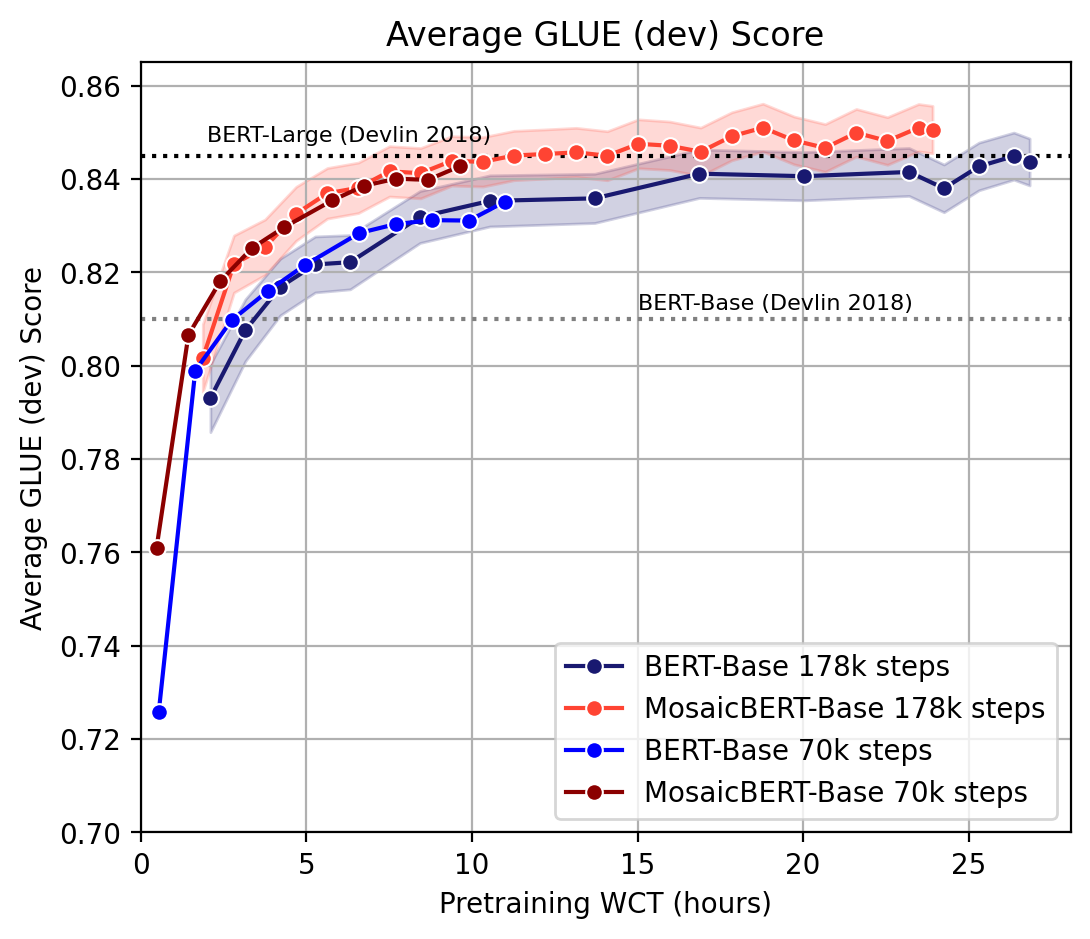
\includegraphics[width=0.7\textwidth]{figures/pareto-comparison-12-28-222pm.png}
    \caption{Pareto curves for BERT-Base and MosaicBERT-Base for runs trained for 70,000 and 178,000 steps with batch size 4096 and sequence length 128. Same data as Figure \ref{fig:intro_figure}B and \ref{fig:bert_large_glue_av}. }
    \label{fig:pareto_comparison}
\end{figure}


\section{Pareto Curves for Benchmarking Neural Network Training}

In order to make meaningful improvements in neural network training efficiency, ML practitioners must be able to compare between different choices of network architectures, hyperparameters, and training algorithms. 
One straightforward way to do this is to characterize the tradeoff between accuracy and training time with a ``tradeoff curve'' or a ``Pareto curve.'' Pareto curves can be generated by varying the length of training for each model configuration; longer training runs take more time but tend to reach higher quality. For a fixed model and task configuration, this method of generating tradeoff curves is an estimate of the theoretical Pareto frontier, i.e. the set of all of the best possible tradeoffs between training time and accuracy, where any further attempt to improve one of these metrics worsens the other. See \citep{mosaicml2022methodology,portes2022fast} for more details.

We therefore consider one model Pareto optimal relative to another if it has superior accuracy across different training budgets while keeping everything fixed. Many studies advertise novel architecture approaches without measuring wall clock time, or simply show an improvement for a single training duration. In this study we show that MosaicBERT-Base is Pareto optimal relative to our BERT-Base baseline for both short training durations and long training durations (Figures \ref{fig:intro_figure}, \ref{fig:bert_base_glue_individual}, \ref{fig:bert_large_glue_av}). We also show that BERT-Large and MosaicBERT-Large are not Pareto optimal relative to BERT-Base and MosaicBERT-Base for training durations under 30 hours (Figure \ref{fig:bert_large_glue_av}).

The Pareto plots in Figures \ref{fig:intro_figure}, \ref{fig:bert_base_glue_individual}, \ref{fig:bert_large_glue_av} and \ref{fig:bert_large_glue_individual} are constructed by taking points from the same runs (with the same learning schedule), instead of having one run per pretraining budget on the plot. We did this for cost reasons; it would have been too expensive to do every run separately. 

For ResNets, it has been established that the most accurate way to generate Pareto curves is to run completely separate training runs for each point on the Pareto curve, where each point also has their own learning rate schedule \citep{portes2022fast}. However, to the best of our knowledge, this has not been clearly established for BERT models. Can Pareto curves for BERT simply be constructed by evaluating checkpoints of a single training run?
%We emphasize that this approximation penalizes intermediate budgets, as they are evaluated with an incomplete learning rate schedule, so we expect that our results would be even stronger had we used the learning rate schedule corresponding to the training time for each point.

Since we ran BERT-Base and MosaicBERT-Base experiments for two separate learning rate schedules (70,000 steps and 178,000 steps with batch size 4096), we can plot the Pareto curves for all of these runs on top of each other (Figure \ref{fig:pareto_comparison}). Somewhat surprisingly, the 70k and 178k curves for BERT-Base (and MosaicBERT-Base) mostly lie on top of each other. This is strong evidence that at least for BERT models, a reasonable Pareto curve can be constructed using checkpoints from a single training run.

We note that the Pareto curve approach discussed here is also related to ``tokens per parameter'' (TPP) considerations that are often discussed in LLM pretraining (e.g. see \citep{dey2023btlm}).




\begin{figure}
    \centering
    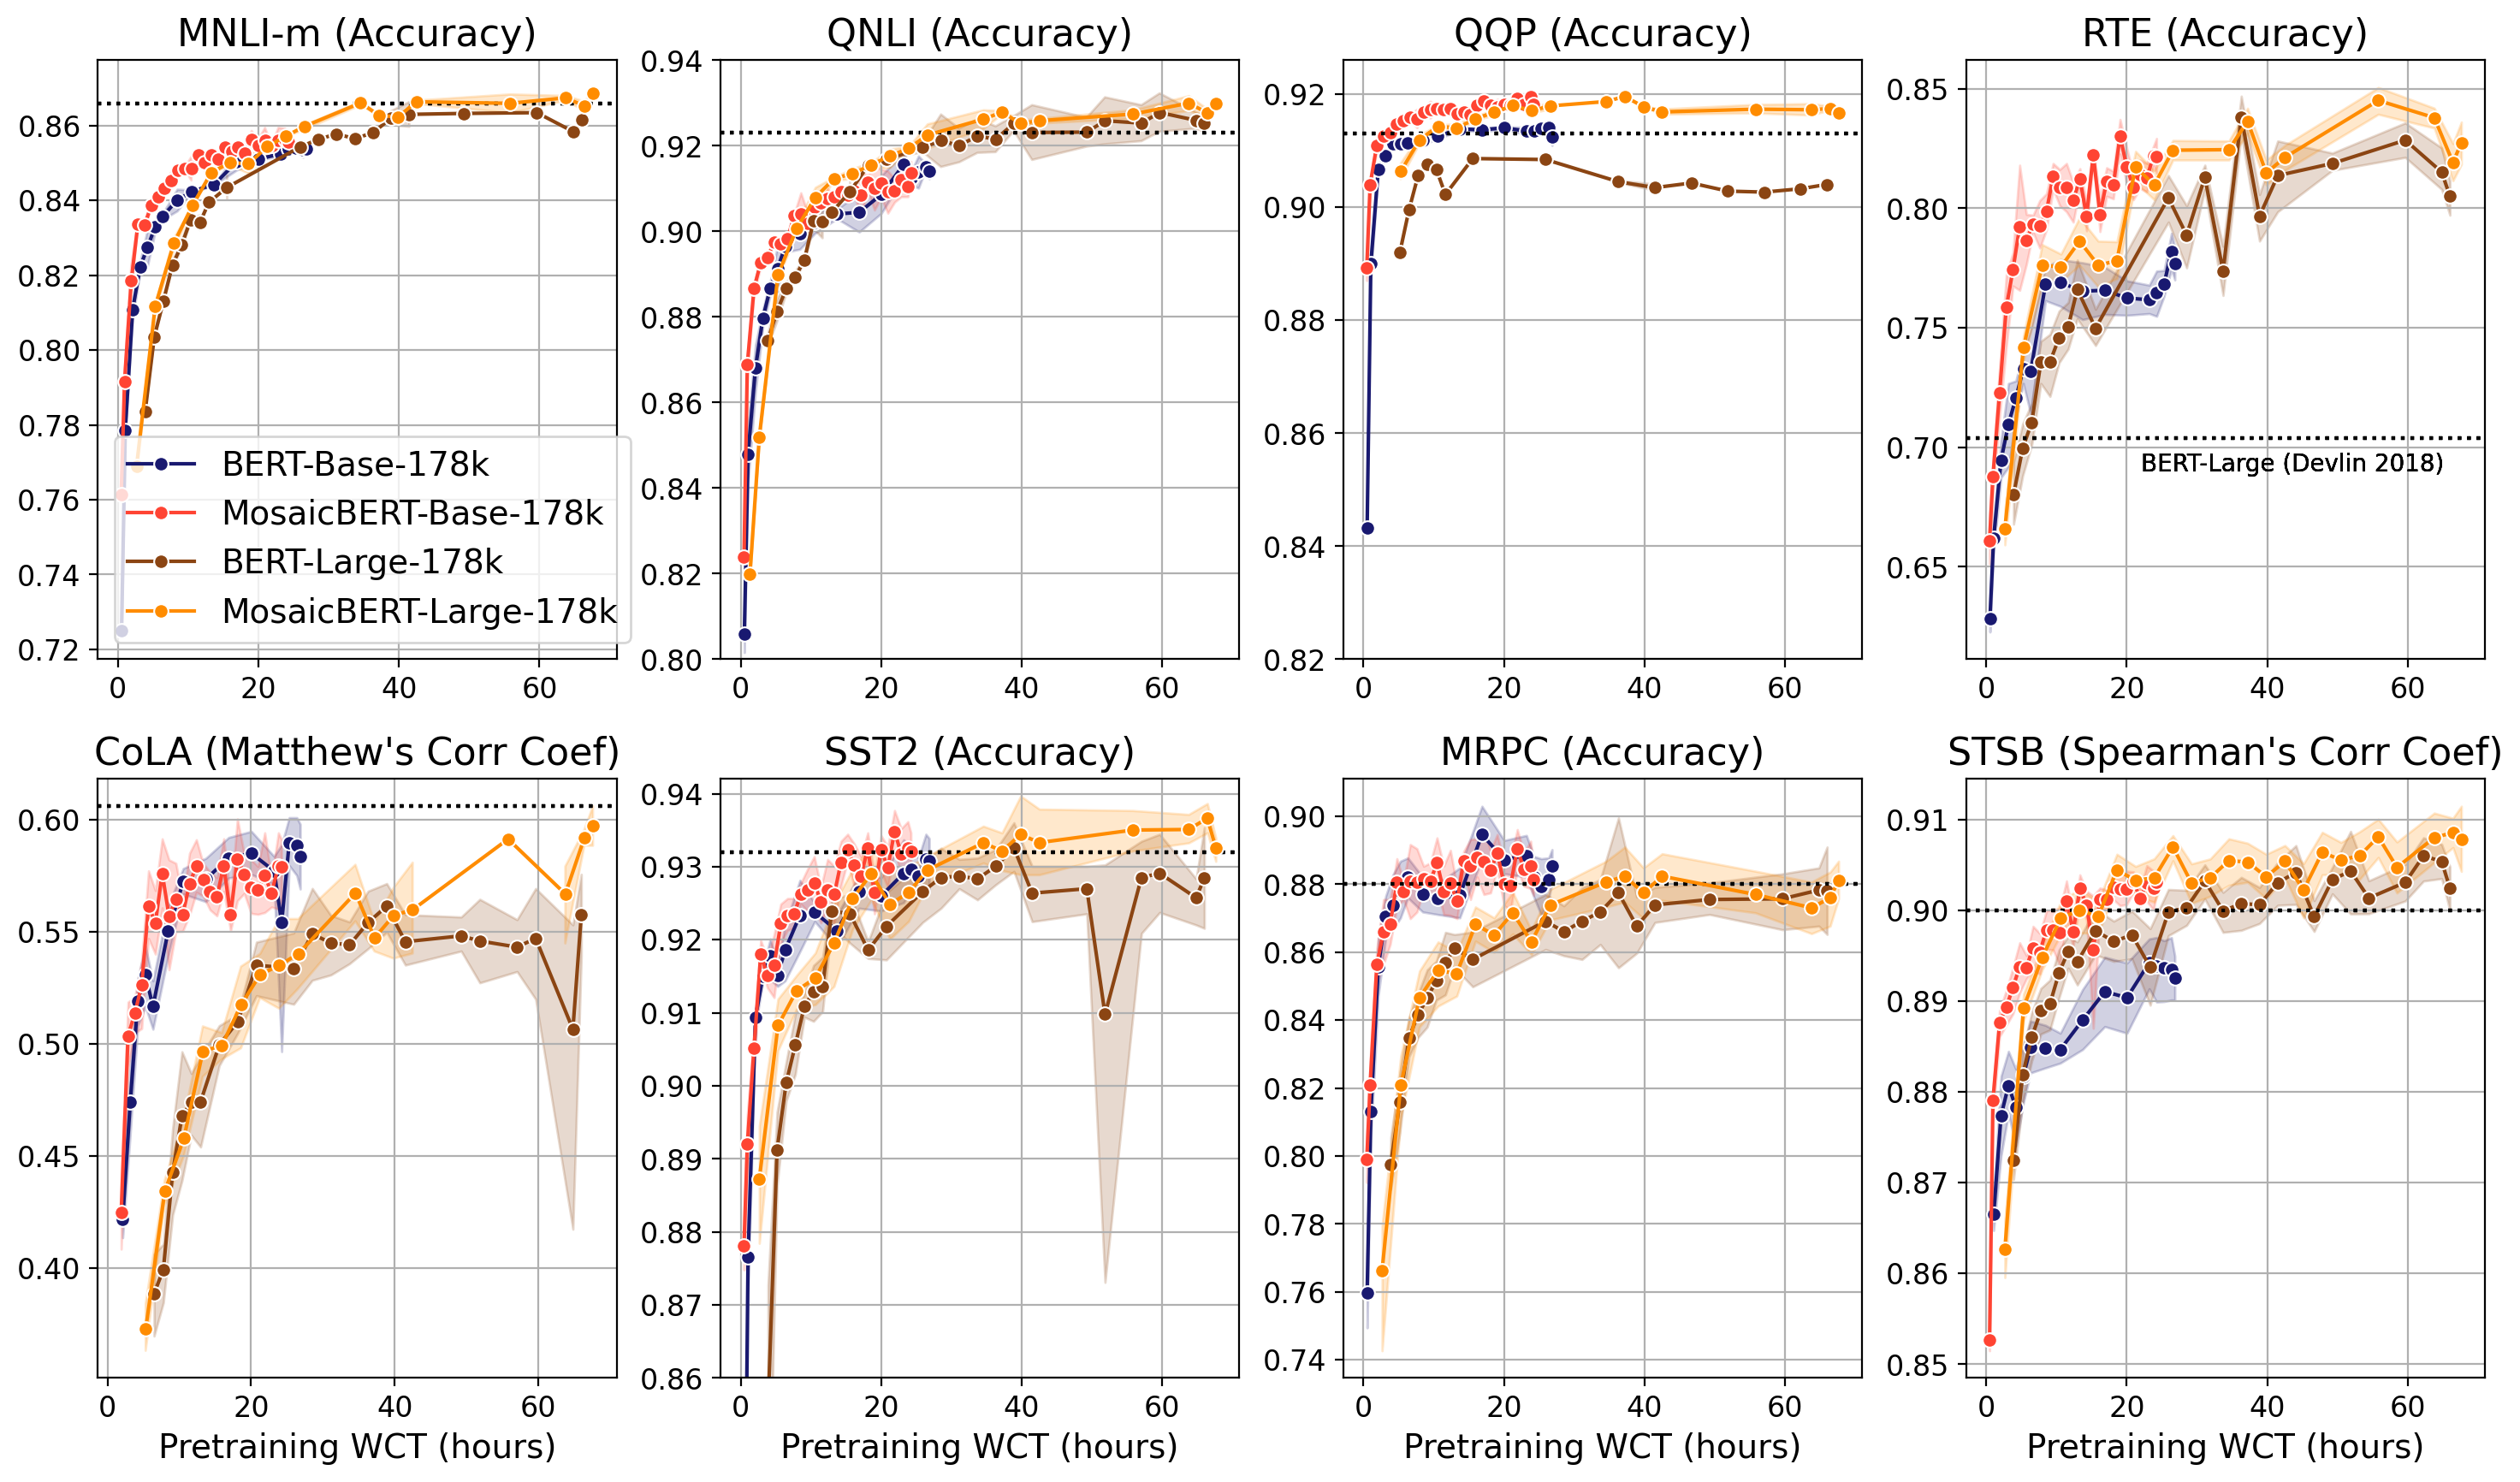
\includegraphics[width=1\textwidth]{figures/bert-large-individual-glue-12-28-145pm.png}
    \caption{MosaicBERT-Base and Large accuracy (dev) vs. pretraining speed Pareto curves for individual GLUE benchmarks. All models were trained on roughly 2 epochs of C4 (178,000 steps with batch size 4096 with maximum sequence length of 128). Error bars represent 95\% confidence interval for n=2-3 pretraining seeds. Dashed black line represents BERT-Large accuracy on the GLUE (dev) data as reported in \cite{liu2019roberta}. The average GLUE score can be found in Figure \ref{fig:bert_large_glue_av}.}
    \label{fig:bert_large_glue_individual}
\end{figure}






\begin{figure}[h!]
    \centering
    \includegraphics[width=0.9\textwidth]{figures/seqlen-glue-av-1-15-832pm.png}
    \caption{MosaicBERT-Base Pareto curves for maximum sequence lengths ranging from 128 to 2048 tokens, with all other hyperparameters fixed. (A) Average GLUE score as a function of pretraining steps. (B) Same data as in A, but with wall clock time on the x-axis. The curve representing a maximum sequence length of 128 tokens is mostly Pareto optimal (red curve). Interestingly, training with batch size and sequence length of \{4096,128\} for 178,000 steps (red curve) leads to the same final average GLUE accuracy \textit{and wall clock time} as training with \{4096, 512\} for 70,000 steps (purple curve). Top dashed line represents BERT-Large average (dev) GLUE score from Devlin et al. 2018, while bottom dashed line represents the BERT-Base average (dev) GLUE score from Devlin et al. 2018 \cite{devlin2018bert}.}
    \label{fig:mosaicbert-base-seqlen}
\end{figure}









\begin{figure}[h!]
    \centering
    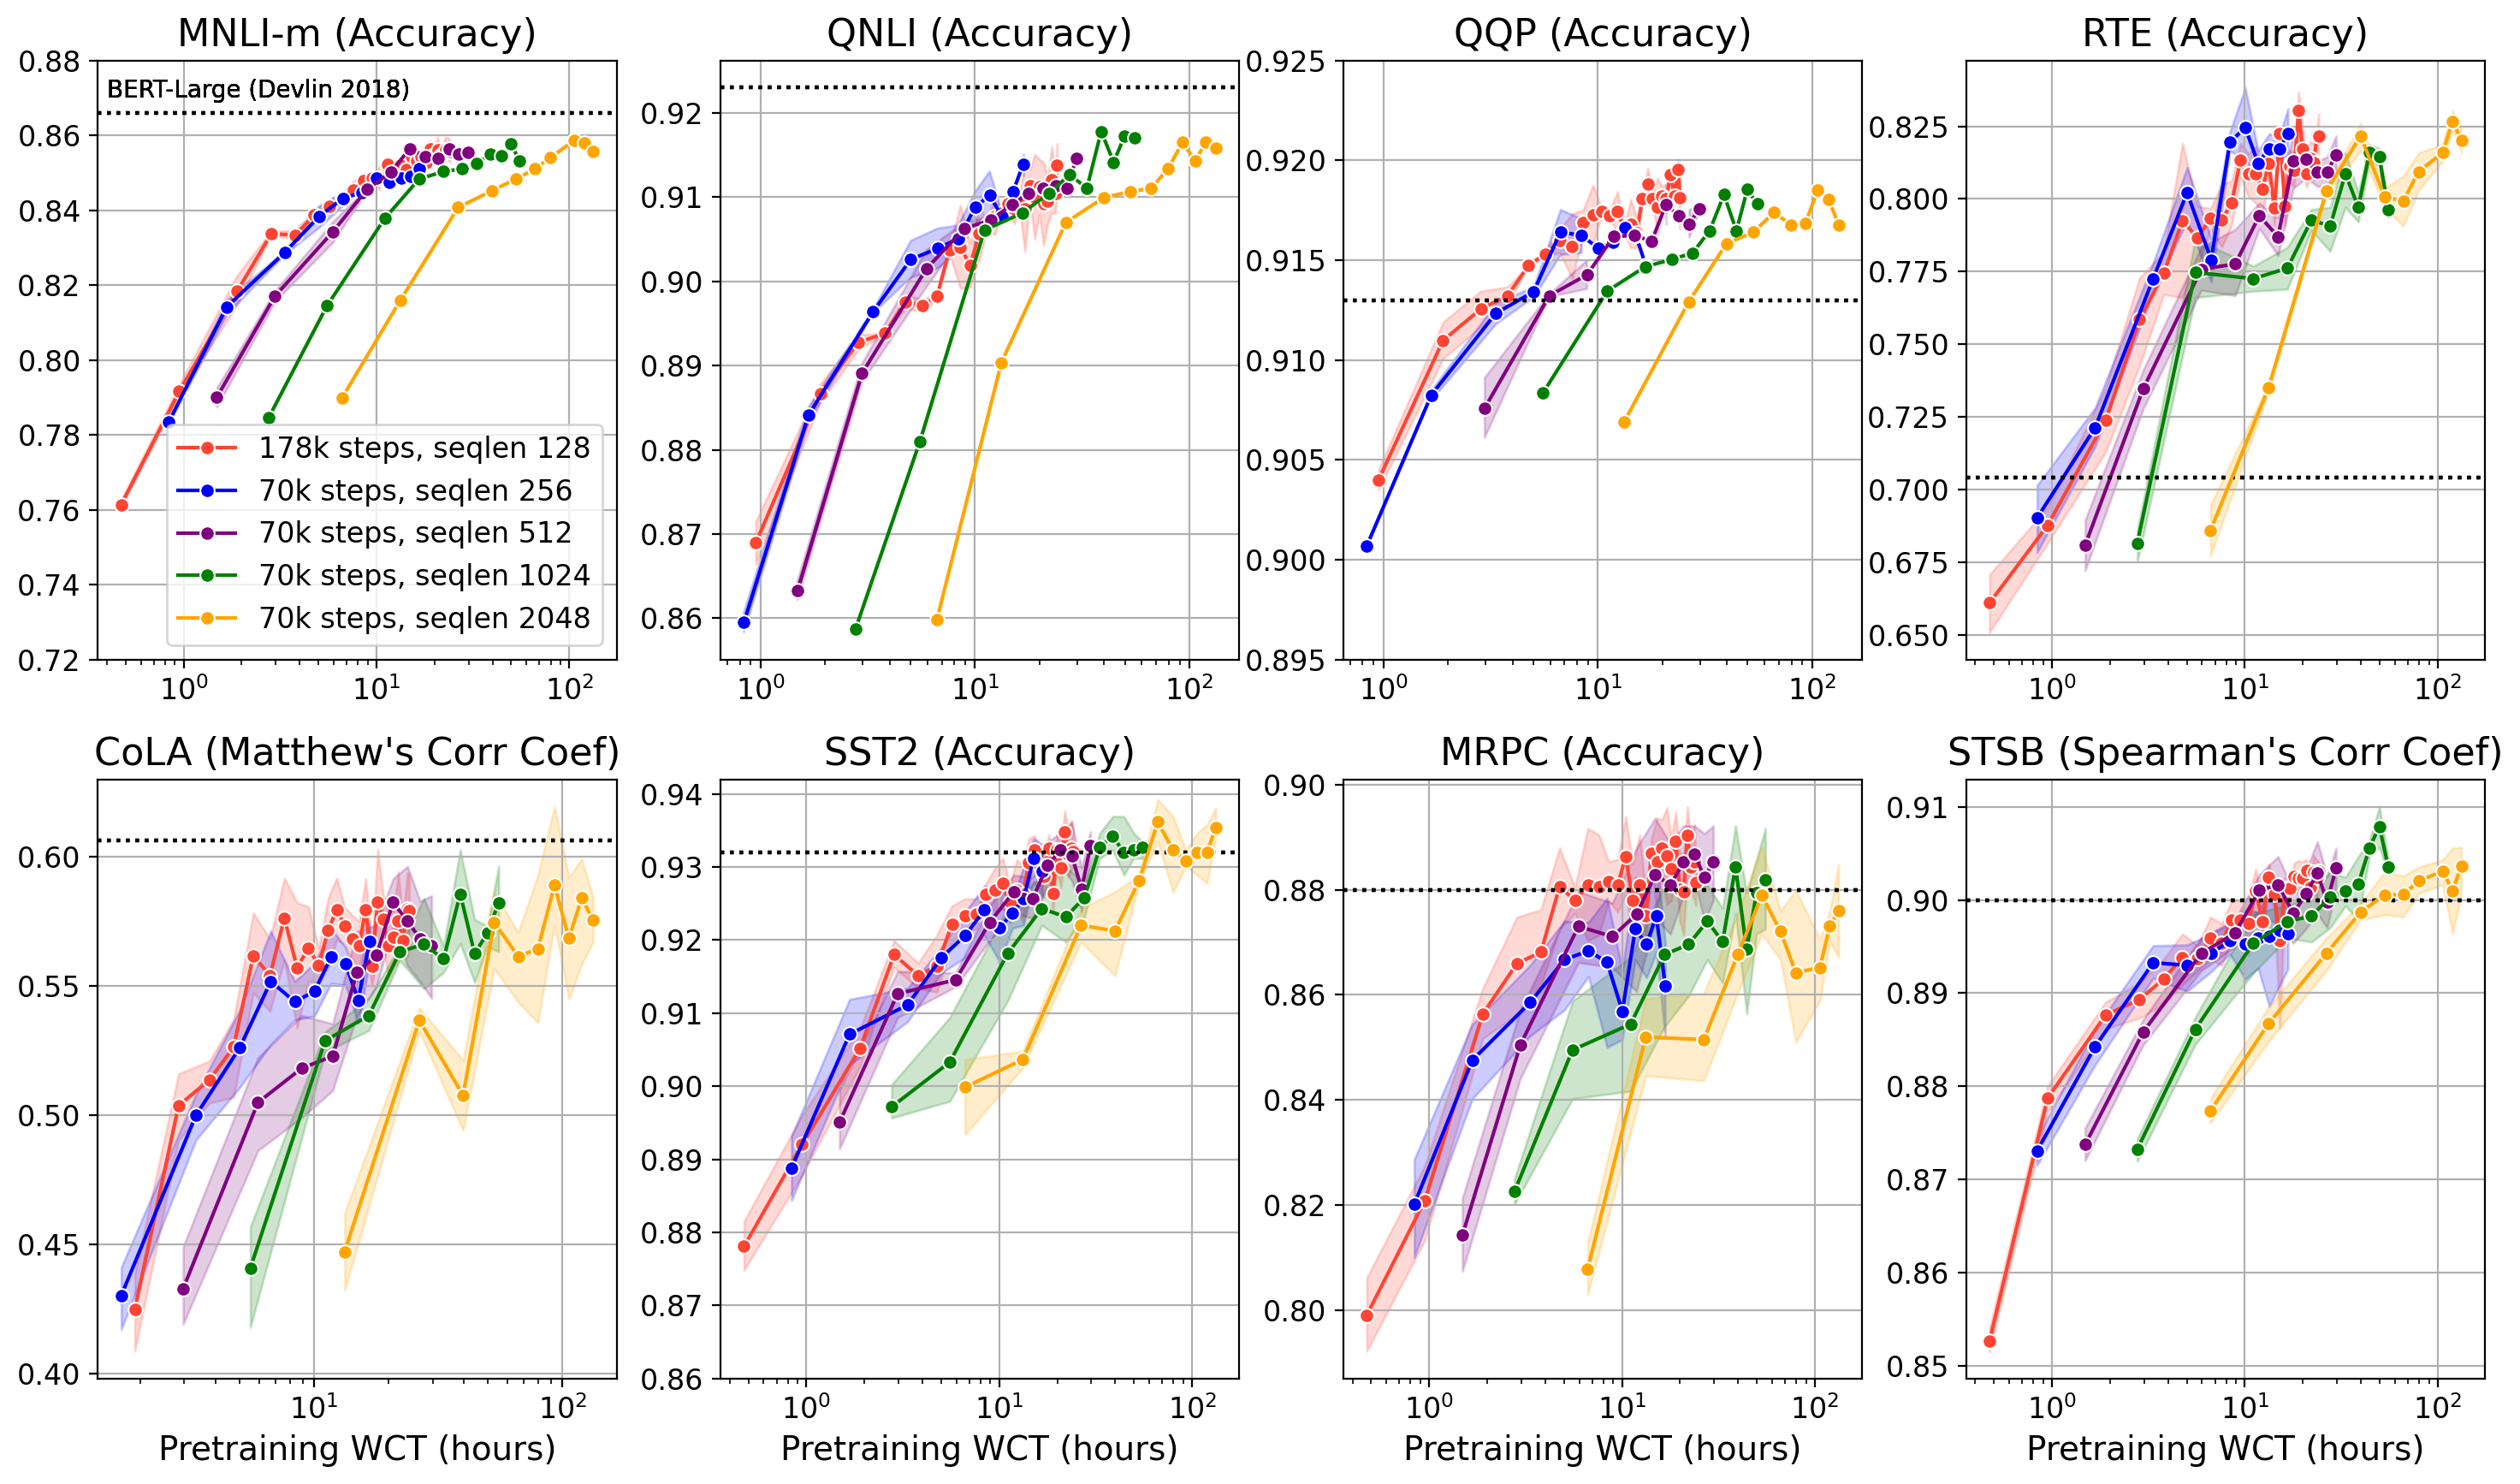
\includegraphics[width=1\textwidth]{figures/seqlen-glue-individual-1-15-823pm.png}
    \caption{MosaicBERT-Base Pareto curves for maximum sequence lengths ranging from 128 to 2048 tokens, with all other hyperparameters fixed. Individual GLUE scores are plotted as a function of pretraining wall clock time. All curves used batch size 4096 and were pretrained for 70,000 steps, except for the curve representing sequence length 128 tokens, which was trained for 178,000 steps (and is the same as MosaicBERT-Base in Figure \ref{fig:bert_large_glue_av}).}
    \label{fig:mosaicbert-base-seqlen-individual}
\end{figure}

\section{MosaicBERT-Base Experiments with Increasing Sequence Length}

Batch size, maximum sequence length, and number of training steps are important hyperparameters that affect both downstream GLUE accuracy as well as wall clock time. While increasing the maximum number of tokens in a sequence leads to a direct increase in wall clock time, it also exposes the model to more data. For example, increasing sequence length from 128 to 256 while keeping all other hyperparameters constant leads to $2\times$ the amount of total training tokens (assuming no padding). However, this will lead to a commensurate increase in pretraining wall clock time. Given our Pareto-based approach, we can therefore ask:\textit{ is it better to train with fewer steps and longer sequence length, or more steps and shorter sequence length? }

Here we find that training for more steps (i.e. 178,000) on shorter sequence length (i.e. 128 tokens) is Pareto optimal for MosaicBERT-Base GLUE scores. 

As part of our experimental benchmarking, we trained MosaicBERT-Base models with varying maximum sequence lengths ranging from 256 tokens to 2048 tokens for 70,000 steps with batch size 4096. We then plotted the downstream GLUE accuracy in Figures \ref{fig:mosaicbert-base-seqlen} and \ref{fig:mosaicbert-base-seqlen-individual}. Besides maximum sequence length, all other pretraining and finetuning hypeparameters are the same as MosaicBERT-Base in the main text (and Tables \ref{tab:pretrain_hyperparams} and \ref{tab:finetuning_hyperparameters}). Each point represents n=1-2 pretraining checkpoints finetuned with multiple seeds according to Table \ref{tab:finetuning_hyperparameters}. The curve representing MosaicBERT-Base trained with sequence length 128 and 178,000 steps is the same as in Figure \ref{fig:bert_large_glue_av}.

When looking at average GLUE accuracy as a function of pretraining steps in Figure \ref{fig:mosaicbert-base-seqlen}A, longer sequence lengths of 256, 512, 1024 and 2048 nominally do better than a maximum sequence length of 128 tokens when trained for 70,000 steps. However, plotting steps on the x-axis can be misleading, as increasing sequence length leads to increased wall clock time (ceteris paribus).

Instead, it is much more informative to plot wall clock time on the x-axis, as in Figure \ref{fig:mosaicbert-base-seqlen}B. Here, the order of the curves is flipped and the curve representing maximum sequence length of 128 tokens is mostly Pareto optimal (red curve). Interestingly, training with batch size and sequence length of \{4096,128\} for 178,000 steps leads to the same final average GLUE accuracy \textit{and wall clock time} as training with \{4096, 512\} for 70,000 steps (purple curve in Figure \ref{fig:mosaicbert-base-seqlen}B). Note that the x-axis here is plotted on a logarithmic scale, as training with sequence length 2048 for 70,000 steps takes more than 100 hours on $8\times$A100 80GB GPUs.

Figure \ref{fig:mosaicbert-base-seqlen-individual} plots the GLUE scores for individual tasks as a function of pretraining wall clock time. The curve representing maximum sequence length of 128 tokens is mostly Pareto optimal (red curve). However, QNLI and STSB seem to benefit from longer maximum sequence lengths.

An important consideration when increasing the maximum sequence length is the issue of padding. Many text samples in our C4 pretraining dataset contained fewer than 2048 tokens and needed to be padded. The ``unpadding'' approach detailed in the main text applies to the feedforward layers of the transformer but not the attention layers. As sequence length is increased, there is potentially wasted computation on padding tokens in the attention layers. This means that wall clock time increases without significant boosts in accuracy. This is likely the case for the curves representing sequence lengths 1024 and 2048. 

Another important consideration is that the GLUE tasks are quite short by modern standards (circa 2023) and contain fewer than 512 tokens. Additionally, all GLUE finetuning in this study was done with maximum sequence length of 256 tokens. Training with sequence length 1024 or 2048 tokens is likely unnecessary for this task. It is possible, however, that these models are superior at tasks that involve long-context dependencies.

The original BERT paper pretrained with a maximum sequence length of 128 tokens for 90\% of training, and then completed pretraining with a sequence length of 512 \citep{devlin2018bert}. The RoBERTa paper pretrained with a maximum sequence length of 512 for the full duration of pretraining and also ``packed'' each batch sample with full sentences up to the limit of 512 tokens to decrease the number of padding tokens \citep{liu2019roberta}.

We released the pretrained checkpoints for these models on the HuggingFace hub in April 2023:
\begin{itemize}
    \item \href{https://huggingface.co/mosaicml/mosaic-bert-base-seqlen-256}{\url{https://huggingface.co/mosaicml/mosaic-bert-base-seqlen-256}}
    \item \href{https://huggingface.co/mosaicml/mosaic-bert-base-seqlen-512}{\url{https://huggingface.co/mosaicml/mosaic-bert-base-seqlen-512}}
    \item \href{https://huggingface.co/mosaicml/mosaic-bert-base-seqlen-1024}{\url{https://huggingface.co/mosaicml/mosaic-bert-base-seqlen-1024}}
    \item \href{https://huggingface.co/mosaicml/mosaic-bert-base-seqlen-2048}{\url{https://huggingface.co/mosaicml/mosaic-bert-base-seqlen-2048}}
\end{itemize}







\begin{table}[h!]
\centering
\footnotesize
\begin{tabular}{p{2.2cm} p{0.5cm} p{0.5cm} p{0.6cm} p{0.6cm} p{0.6cm} p{0.6cm} p{0.6cm} p{0.6cm} p{0.6cm} p{0.6cm} p{0.6cm} p{0.6cm} p{0.6cm}}

\toprule
\textbf{Model} & \textbf{Bsz} & \textbf{Steps} &\textbf{SeqL} & \textbf{MNLI} & \textbf{QNLI} & \textbf{QQP} & \textbf{RTE} & \textbf{SST} & \textbf{MRPC} & \textbf{CoLA} & \textbf{STS} & \textbf{Av.} \\
\midrule
\textbf{BERT-Large} BookC + Wiki & 256 & 1M & 128 & 86.6 & 92.3 & 91.3 & 70.4 & 93.2 & 88 & 60.6 & 90 & 84.05 \\ 
\textbf{RoBERTa-Base} all data+500k & 8k & 500k & 512 & 87.6 & 92.8 & 91.9 & 78.7 & 94.8 & 90.2 & 63.6 & 91.2 & 86.35 \\ 
\textbf{RoBERTa-L}: & & & & & & & & & & & & \\ 
1. BookC+Wiki & 8k & 100k & 512 & 89 & 93.9 & 91.9 & 84.5 & 95.3 & 90.2 & 66.3 & 91.6 & 87.8 \\ 
2. all data & 8k & 100k & 512 & 89.3 & 94 & 92 & 82.7 & 95.6 & 91.4 & 66.1 & 92.2 & 87.9 \\ 
3. all data+300k & 8k & 300k & 512 & 90 & 94.5 & 92.2 & 83.3 & 96.1 & 91.1 & 67.4 & 92.3 & 88.4 \\ 
4. all data+500k & 8k & 500k & 512 & 90.2 & 94.7 & 92.2 & 86.6 & 96.4 & 90.9 & 68 & 92.4 & 88.9 \\ 
\midrule
\textbf{BERT-Base} & 4k & 178k & 128 & 85.4 & 91.6 & 91.4 & 78.2 &  93.10 & 89.5 & 59 & 89.4 &    84.7 \\
 \textbf{MosaicBERT-B} & 4k & 178k & 128 & 85.6 & 91.4 & 92 & 83 &  93.5 & 89 & 58.2 & 90.3 &    85.4 \\
\textbf{BERT-Large} & 4k & 178k & 128 & 86.3 & 92.8 & 90.9 & 83.8 &  93.3 & 87.8 & 56.2 & 90.6 &    85.2 \\
\textbf{MosaicBERT-L} & 4k & 178k & 128 & 86.9 & 93 & 92 & 84.5 &  93.7 & 88.2 & 59.7 & 90.9 &    86.1 \\
\bottomrule
\end{tabular}
\label{roberta_table}
\caption{Model performance comparison on GLUE (dev) tasks. Data from Table 8 of the RoBERTa paper \citep{liu2019roberta}. Values for BERT and MosaicBERT in bottom rows are best average values per task from Figure \ref{fig:bert_large_glue_individual}.}
\label{tab:roberta}
\end{table}



\section{Comparison to RoBERTa}

As mentioned in the main text, RoBERTa (``Robustly optimized BERT approach'') was an important follow-up to the original BERT \citep{liu2019roberta}. In this study, they kept the exact BERT architecture the same but changed the \textit{training recipe} by removing the next sentence prediction (NSP) objective, training for longer on much larger datasets, and changing the batch size, among other things. Many of the training choices in RoBERTa have become standard practice; our training recipe therefore more closely resembles RoBERTa than the original BERT. The RoBERTa paper also did careful experiments and ablations that were helpful for the research community.

The main pretraining results from RoBERTa-Base and Large are shown in Table \ref{roberta_table} (data from Table 8 in the Appendix of the RoBERTa paper \citep{liu2019roberta}). In particular, they trained on:
\begin{enumerate}
    \item BookCorpus \citep{zhu2015aligning} and English Wikipedia for 100k steps with batch size 8192 and sequence length 512
    \item BookCorpus  \citep{zhu2015aligning} and English Wikipedia (16GB), plus ``additional data'' CC News, the English portion of the CommonCrawl News dataset (76GB) \citep{nagel2016common}, OpenWebText Corpus (38GB) \citep{Gokaslan2019OpenWeb}, and STORIES (31GB) \citep{trinh2018simple} for 100k steps with batch size 8192 and sequence length 512
    \item The full dataset mixture (160GB) for 300k steps with batch size 8192 and sequence length 512
    \item The full dataset mixture (160GB) for 500k steps with batch size 8192 and sequence length 512
\end{enumerate}

The RoBERTa-Base and Large values are better than the MosaicBERT-Base and Large values.  An apples-to-apples comparison of RoBERTa and MosaicBERT experiments would keep all hyperparameters consistent, including training data and batch size. Since we cannot do this post hoc, a somewhat reasonable comparison would be to keep the total amount of data constant. 100k steps with batch size 8192 is roughly equivalent to 178k steps with batch size 4096 (i.e. it is almost equivalent to 89k steps with batch size 8192). However, RoBERTa also pretrained with a maximum sequence length of 512 tokens,\textit{ which is $4\times$ longer than the maximum sequence length of 128 we used for pretraining in this study}. This means that the ``worst'' RoBERTa models trained with batch size 8192 for 100k steps still saw $4\times$ more tokens than the MosaicBERT models trained with batch size 4096 for 178k steps.  This is one likely one reason that the final RoBERTa values on GLUE are higher. 

Additionally, the RoBERTa study formatted the data to minimize padding tokens by packing each sample with full sentences sampled contiguously from one or more documents (with an extra separator token) \cite{liu2019roberta}. They also did a learning rate sweep for single-task GLUE finetuning \{1e-5, 2e-5, 3e-5\}, which we did not do. Finally, the differences between MosaicBERT and RoBERTa could also be due to differences in the underlying datasets.










%\section{Ablation Experiment Details}

\section{GLUE Benchmark Details}
\label{sec:glue-details}

The GLUE benchmark consists of 8 (originally 9) tasks \citep{wang2018glue}.
Since there has been a Cambrian explosion of benchmarks since the halcyon days of GLUE, we elaborate on the individual GLUE benchmarks for reference. We used the GLUE tasks from HuggingFace for finetuning and evaluation: \href{https://huggingface.co/datasets/glue}{\url{https://huggingface.co/datasets/glue}}. All evaluation was done on the validation (a.k.a. dev) splits.

\subsection{Large Finetuning Datasets}

\textbf{MNLI (Multi-Genre  Natural  Language  Inference) }[392,702 train | 19,643 validation | 19,643 test]  is a large crowd-sourced entailment classification task \citep{williams2017broad}.  The model is given two sentences and has to predict whether the second sentence is entailed by, contradicts, or is neutral with respect to the first one. For example:
\begin{itemize}
    \item Premise: "Buffet and a  la carte available."
    \item Hypothesis: "It has a buffet."
    \item Label: 0 (entailment)
\end{itemize}

MNLI has two subsets, ``matched'' (MNLI-m) and ``mismatched'' (MNLI-mm). All numbers reported in this study are for MNLI-m, unless otherwise stated.

\textbf{QNLI} [104,743 train | 5,463 validation | 5,463 test] this Stanford Question Answering dataset consists of question-paragraph pairs drawn from Wikipedia \citep{rajpurkar2016squad}.

\textbf{QQP (Quora Question Pairs 2) }[363,846 train | 40,400 validation | 390,965 test]. The task is to determine whether two sentences are semantically equivalent \citep{Iyer2017Quora}.

\subsection{Small Finetuning Datasets}

\textbf{RTE (Recognizing Textual Entailment) }[2,490 train | 277 validation | 3,000 test] Given two sentences, the model has to predict whether the second sentence is or is not entailed by the first sentence \citep{dagan2006pascal,giampiccolo2007third,bentivogli2009fifth}. Note that in our work we use a checkpoint from the MNLI finetuning to finetune on RTE.

\textbf{CoLA (Corpus of Linguistic Acceptability)} [8,551 train | 1,040 validation | 1,063 test] \citep{warstadt2019neural} is a benchmark with sentences that are either linguistically acceptable or grammatically incorrect. For example: 
\begin{itemize}
    \item "The higher the stakes, the lower his expectations are." Label: 1 (acceptable)
    \item "Mickey looked up it." Label: 0 (unacceptable)
\end{itemize}

\textbf{SST-2 (Stanford Sentiment Treebank)} [67,349 train | 872 validation | 1,821 test] consists of sentences from movie reviews. The task is to classify the sentiment as either positive or negative \citep{socher2013recursive}.



\textbf{MRPC (Microsoft Research Paraphrase Corpus)}[3,668 train | 408 validation | 1,725 test] \citep{dolan2005automatically} The dataset consists of sentence pairs extracted from online news sources. The task is to classify whether the sentences in the pair are semantically equivalent.

\textbf{STSB (Semantic Textual Similarity Benchmark) }[5,749 train | 1,500 validation | 1,379 test] This dataset contains sentence pairs that are given similarity scores from 0 to 5 \citep{cer2017semeval}.

Note that we excluded finetuning on the 9th GLUE task WNLI (Winograd NLI) \citep{levesque2012winograd}, as in the original BERT study (it is a very small dataset [634 train, 146 test] with a high number of adversarial examples). Finetuning on RTE, MRPC and STSB starts from a checkpoint already finetuned on MNLI (following the example of \cite{izsak2021train} and other studies). This is done because all the above tasks deal with sentence pairs, and this staged finetuning leads to consistent empirical improvement.



\section{MosaicBERT-Large Multinode Throughput Scaling}

The experiments in the main section of this paper were all performed on a single node with $8\times$A100 GPUs. How well do our innovations to the BERT architecture maximize throughput at the multinode scale?

We measured the throughput of MosaicBERT-Large (430M) during training on 8, 16, 32, 64, 128 and 200 GPUs, and plotted the tokens per second for various global batch sizes. Global batch size is an important factor in the throughput measurements; in general, cranking up the batch size increases the GPU utilization and raw throughput. As the number of nodes increases, the global batch size needs to be increased as well in order to maintain high throughput.

If the global batch size is kept constant while increasing the number of nodes, the throughput does not increase linearly. This can be seen in Figure \ref{fig:bert-large-throughput}; a global batch size of 4096 spread across 64 GPUs using Distributed Data Parallelism (DDP) means that each GPU will only apply matmul operations on matrices with a dimension of 64, which leads to suboptimal throughput. If the global batch size is increased to 65,536 across 64 GPUs, this roughly means that each GPU will apply matmul operations on matrices with a dimension of 1024, leading to higher throughput. However, such a large global batch size might not lead to the best downstream accuracy; this is a question that we were not able to address in this study due to resource and time constraints.

\subsection{How MosaicBERT modifications might scale to larger models}
All of the architectural and configuration choices made in MosaicBERT can in principle be applied to larger models, although they might have different effects on throughput. Additionally, they should not pose any issues with different forms of parallelism (some of the modifications we explored were used successfully at large scale in frameworks like MEGATRON as well as MPT-7B and MPT-30B \citep{MosaicML2023IntroducingMPT7B,MosaicML2023IntroducingMPT30B}). For example, Gated Linear Units should have no issues with tensor parallelism as long as the matrix multiplications are a multiple of the Tensor Parallel world size. As models are scaled, LayerNorm becomes a smaller portion of the total compute, so low precision LayerNorm might not matter as much.



\begin{figure}[h!]
    \centering
    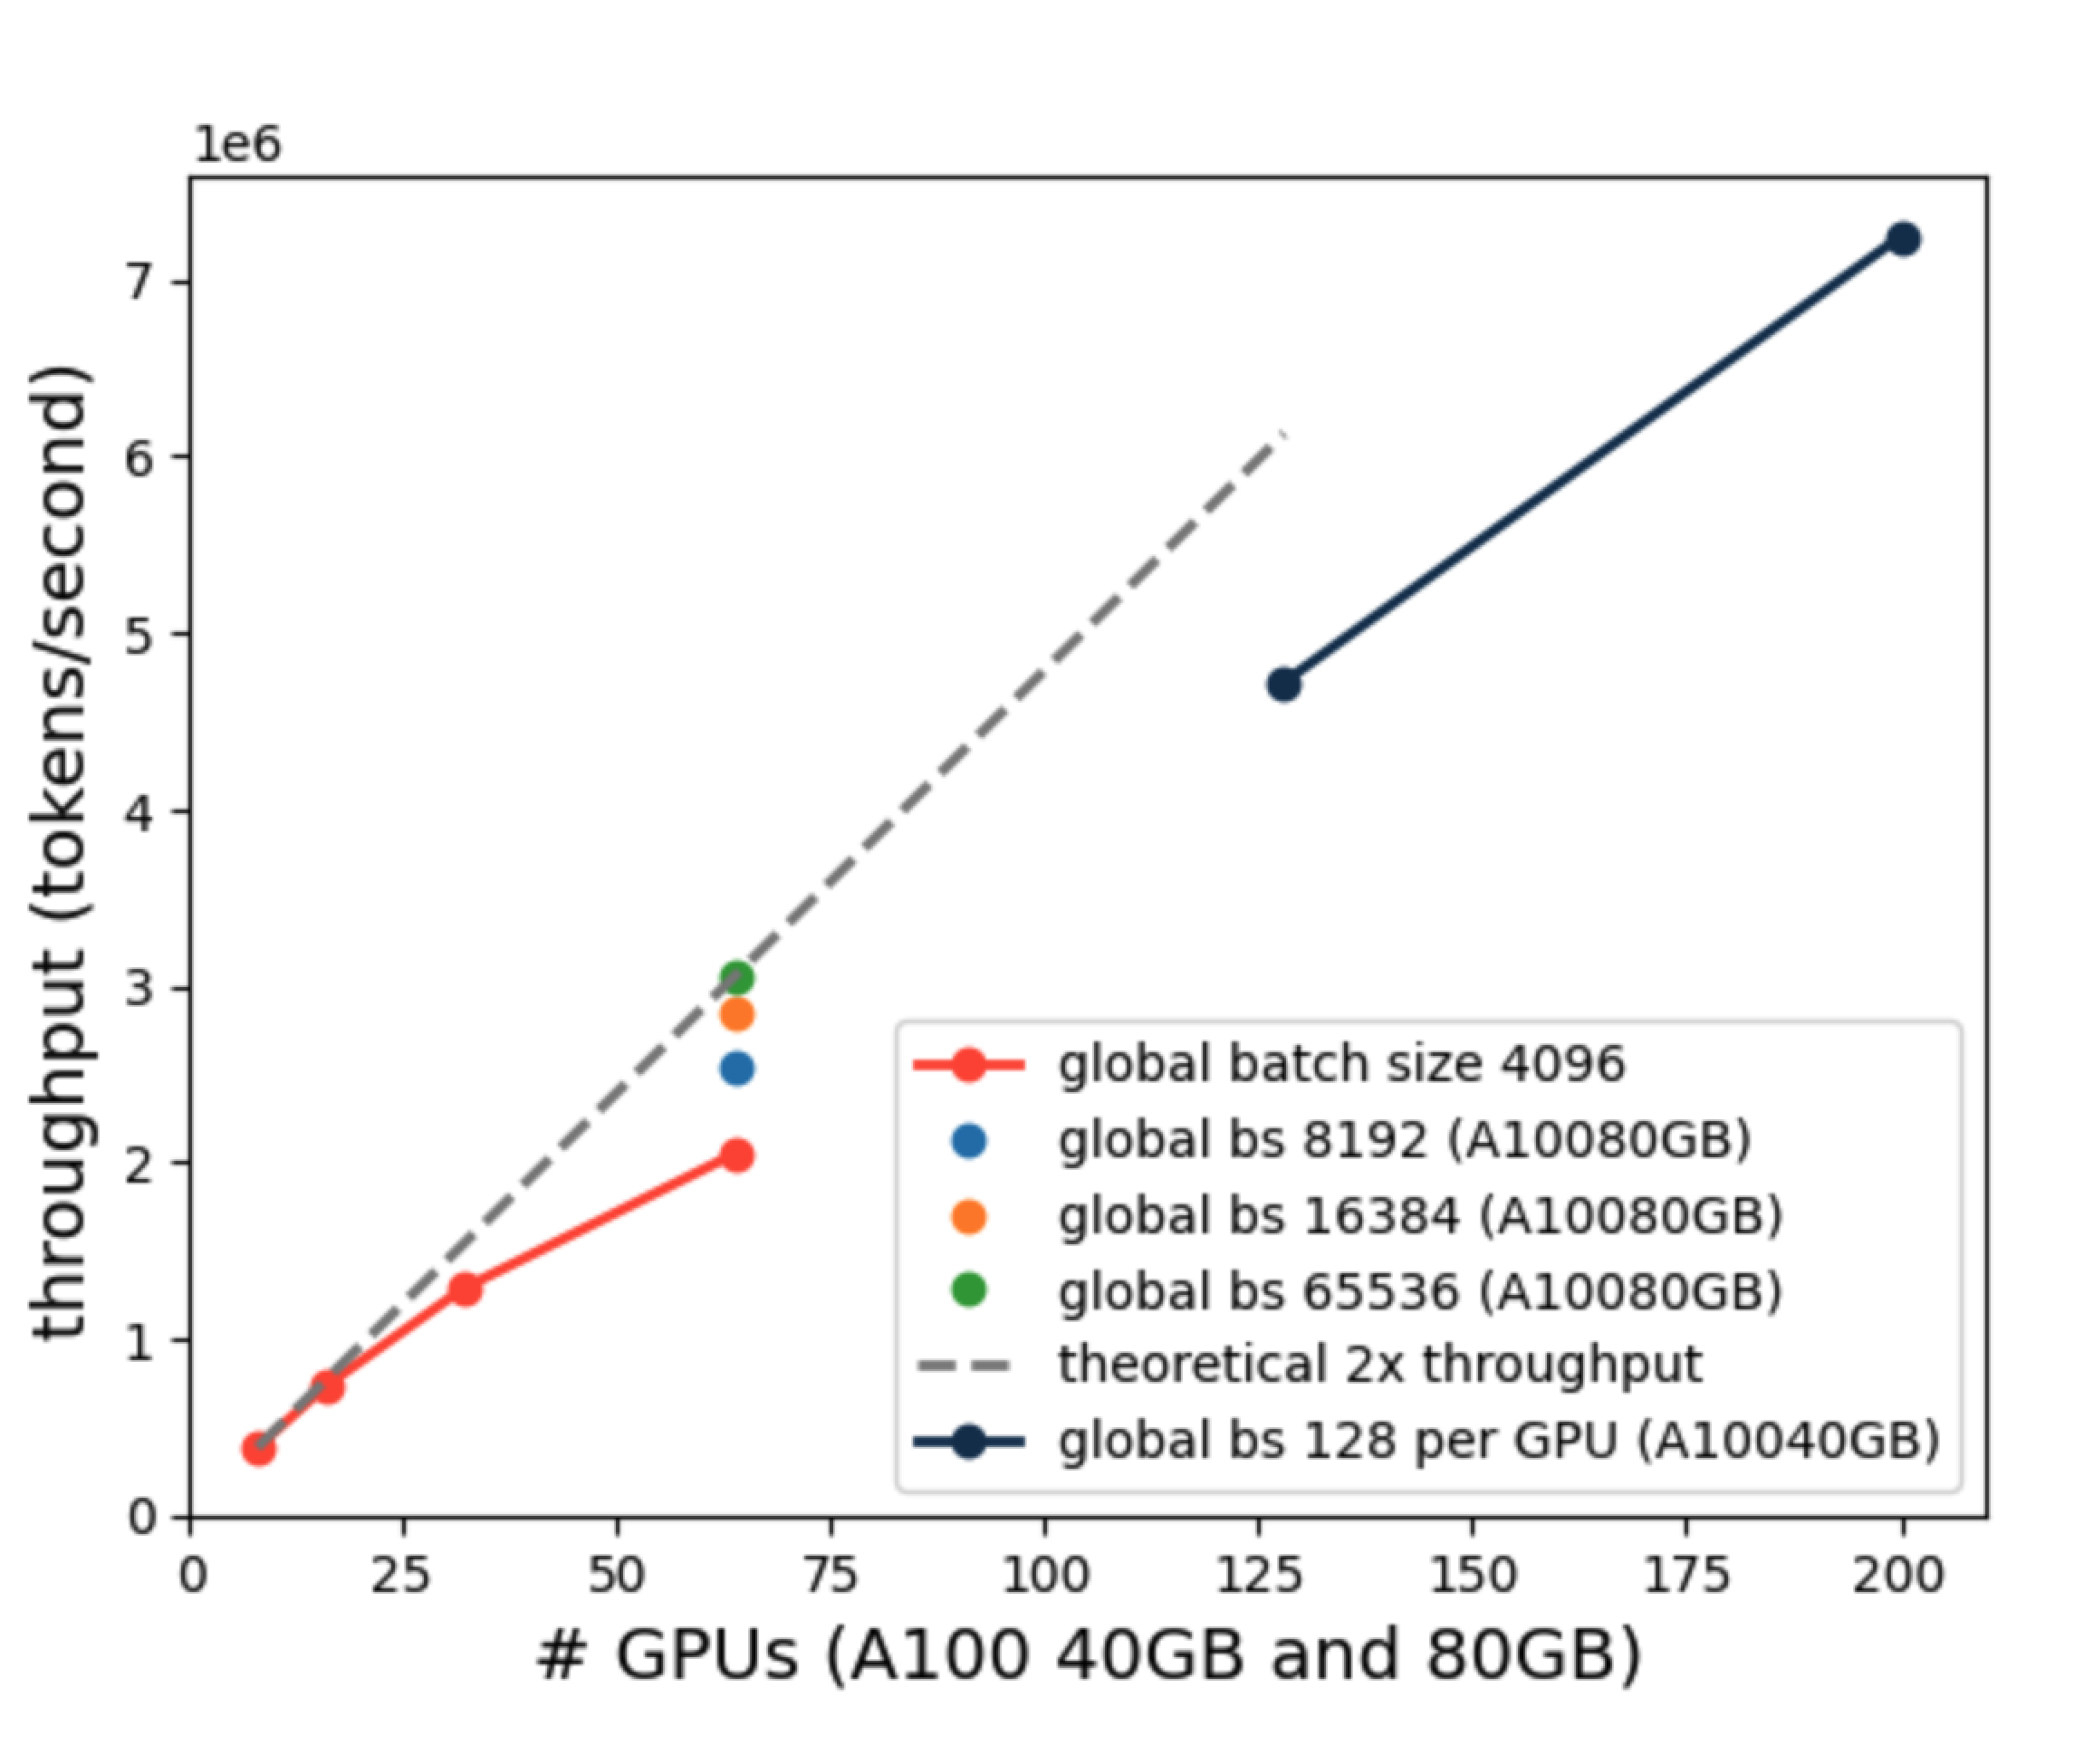
\includegraphics[width=0.5\textwidth]{figures/rapid-bert-large-throughput.png}
    \caption{MosaicBERT-Large (430M) multinode throughput scaling}
    \label{fig:bert-large-throughput}
\end{figure}






\section{MosaicBERT-Base Model FLOPs Utilization (MFU)}

Model FLOPs Utilization (MFU) is an estimate of what percentage of the hardware's FLOPs are being used during training.  The estimate is based on the measured throughput and the known FLOPs of the computation.

MFU calculates the utilization from the floating point operations required for a single forward/backwards pass of the model, and does not account for the additional compute required for other implementation details such as activation checkpointing. Thus, MFU is independent of implementation and hardware. For more details, see \cite{korthikanti2022reducing}. All FLOP calculations exclude the operations required for normalization, activation, and residuals.


Following the notation in the PaLM paper \citep{chowdhery2022palm}, Model FLOPs Utilization (MFU) is approximated as:

\begin{equation}
    \textrm{MFU} = \frac{(6 \cdot n_{parameters} \cdot T_{observed})}{n_{gpus} \cdot T_{theoretical}}
\end{equation}

where $T_{observed}$ is the observed throughput and $T_{theoretical}$ is the theoretical peak throughput.

In the numerator, the number of learnable parameters in the model is multiplied by a factor of 6 to estimate the matmul FLOPs per token seen ($2\times$ for the forward pass and $4\times$ for the backward pass). This is then multiplied by the number of tokens seen per second. As a first-order approximation, we exclude the extra FLOPs per token due to dense self-attention.

In the denominator, the theoretical peak throughput is provided in the GPU hardware specs. For A100 GPUs using \texttt{bfloat16}, this theoretical peak throughput is 312 teraFLOPs.

% \textbf{TODO: add more details an caveats here (e.g. that we are including padded tokens in the calculation)}



\begin{table}[]
\begin{tabular}{p{2.3cm} p{1.8cm} p{1.0cm} p{1.2cm} p{2.cm} p{1.cm} p{1.7cm}}
\toprule
Model & Throughput (tokens /sec) & MFU & Hardware & Time to 79.6 & Batch Size & Microbatch Size \\ \midrule
BERT Base & 0.4e6 & 10.4\% & 8$\times$ A100 80 & 110.4 minutes (1.84 hours) & 4096 & 512 \\
MosaicBERT Base & 1.1e6 & 39.97\% & 8$\times$ A100 80 & 67.8 minutes (1.13 hours) & 4096 & 512 \\
MosaicBERT Base & 0.938e6 & 30.9\% & 8$\times$ A100 40 & 76.8 minutes & 4096 & 128 \\
MosaicBERT Base & 1.88e6 & 31.0\% & 16$\times$ A100 40 & 38.5 minutes & 4096 & 128 \\
MosaicBERT Base & 3.15e6 & 25.9\% & 32$\times$ A100 40 & 23.1 minutes & 4096 & 128 \\
MosaicBERT Base & 4.77e6 & 19.6\% & 64$\times$ A100 40 & 15.7 minutes & 4096 & 64 \\
\bottomrule
\end{tabular}
\caption{Multinode Throughput scaling for MosaicBERT-Base}
\end{table}



















\begin{table}[h!]
\centering
\begin{tabular}{p{2.5cm}p{2cm}p{3cm}p{2cm}p{2.5cm}}
\toprule
MosaicBERT-Base Av. GLUE Score & $8\times$A100 80GB hours & $8\times$A100 80GB cost (\$2.50 GPU/hr) & $8\times$A100 40GB hours & $8\times$A100 40GB cost (\$2 GPU/hr) \\
\midrule
79.6 & 1.13 & \$22.60 & 1.28 & \$20.00 \\

82.2 & 2.81 & \$56.20 & 3.19 & \$51.00 \\

83.4 & 5.27 & \$105.40 & 5.99 & \$95.78 \\
\bottomrule
\end{tabular}
\caption{MosaicBERT-Base GLUE (dev) scores, time and cost comparison}
\label{table:cost-estimate-MosaicBERT-base}
\end{table}


\section{GPU Pricing}

As of mid-2023, A100 GPU pricing ranges from \$4.10 (40 GB) for on demand cloud compute on AWS, to \$2.46 (40 GB) / \$5.00 (80 GB) per GPU on GCP to \$1.10 (40 GB) / \$1.50 (80 GB) per GPU using Lambda labs. At an intermediate price of \$2.50 an hour per A100 80 GB GPU, training to 79.6 GLUE average score takes 1.13 hours and costs roughly \$22.60.\footnote{See for example ``Cloud GPU instances with the largest VRAM 2022'' \href{https://medium.com/@aleixlopez/cloud-gpu-instances-to-solve-out-of-memory-error-2022-d5012883a272?}{(\url{medium.com/@aleixlopez/cloud-gpu-instances-to-solve-out-of-memory-error-2022-d5012883a272?)}}} Some example costs are calculated in Table \ref{table:cost-estimate-MosaicBERT-base}.



\section{Gated Linear Units (GLU) Optimizations}

GLU adds elementwise multiplication of two linear projections and it leads to qualitative improvements over the standard Transformer block. There are multiple ways to implement GLUs and we experimented with two implementations. Figure \ref{fig:glu-diagrams} shows standard feedforward transformer block (A) and two implementations of GLUs (B-C). ``Fused GLU'' in (C) fuses the two matrix multiplications into one and is expected to perform better in some domains. 

\begin{figure}
    \centering
    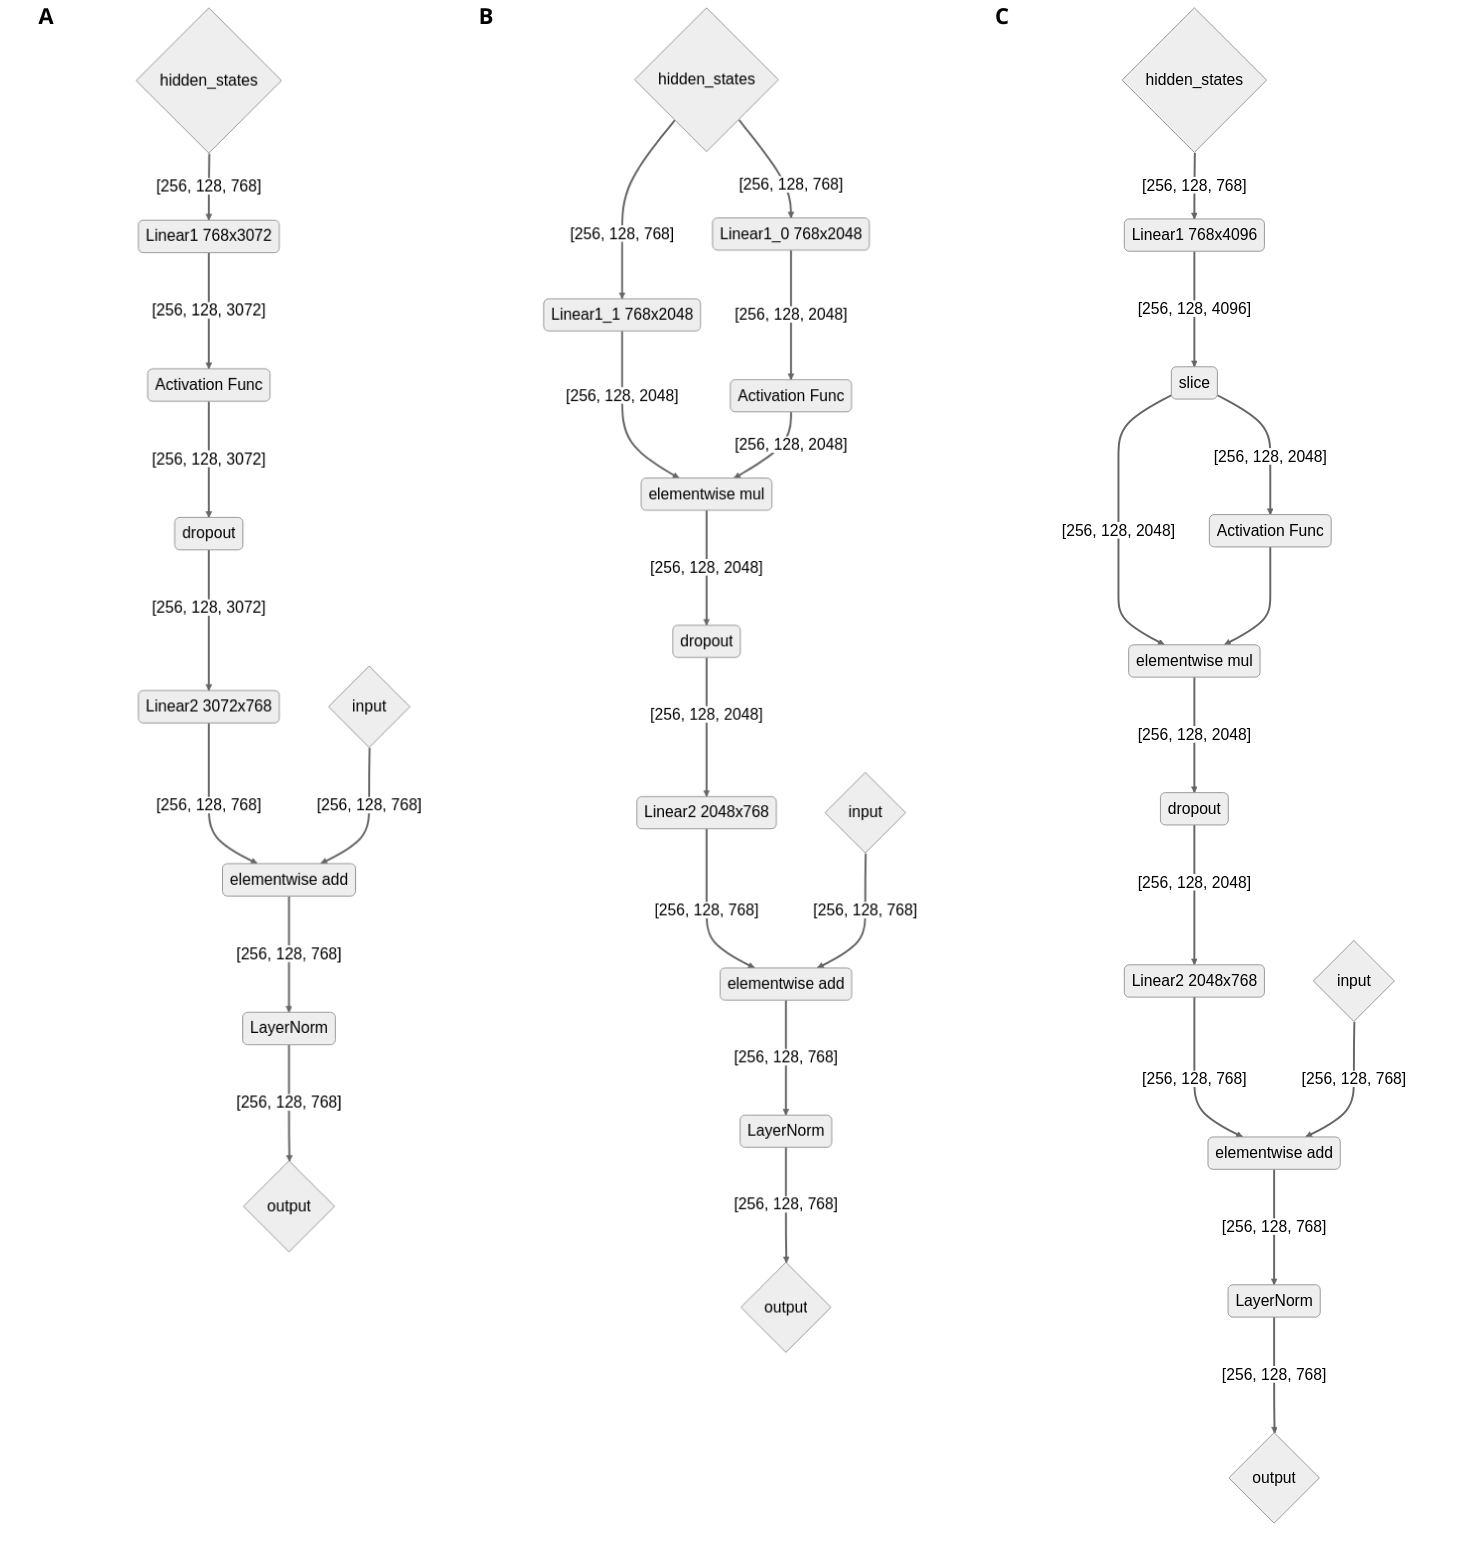
\includegraphics[width=1\textwidth]{figures/glu-diagrams.png}
    \caption{Standard FeedForward Transformer Block and Gated Linear Unit Modifications. Each edge shows the tensor dimension with a batch size of 256, sequence length of 128 and a hidden dimension of 768. (A) A standard transformer feedforward block. (B) Naive implementation of a Gated Linear Unit. The number of parameters in this are the same as in (A). (C) Fused implementation of a Gated Linear Unit where the two matrix multiplications (\texttt{Linear1\_0} and \texttt{Linear1\_1}) from (B) are fused into one (\texttt{Linear1}) with $2\times$ the parameters. Here the output is sliced, and is functionally equivalent to (B).}
    \label{fig:glu-diagrams}
\end{figure}

Figure \ref{fig:glu-slowdown} shows the performance impact of the two GLU over standard feedforward transformer block (which would be $0\%$ slowdown) for a single GPU. This figure only shows the performance of the forward pass, and the backward pass is expected to behave similarly. We can draw two conclusions from this chart: 1) For smaller batch sizes, both GLU implementations add significant overhead over the standard block 2) For batch sizes $<128$, Fused GLU implementation is better than regular GLU implementation and beyond 128 it's slightly worse. The implementation used in the main text is the ``Fused GLU'' implementation (C) with global batch size 4096. Since the profiling in Figure \ref{fig:glu-slowdown} is per GPU, this is in the regime of $4096/8=512$.

The main reason for slowness of GLUs over standard block is extra elementwise multiplication in GLU layers. As for why fused implementation is slower, profiling analysis shows that the Linear layer ends up calling different CUDA kernels for matrix-multiplications and their relative performance varies for different sizes. While the MosaicBERT architecture in this work uses the fused GLU implementation, the analysis here indicates that it would be slightly more efficient to use the standard GLU implementation instead.

\begin{figure}
    \centering
    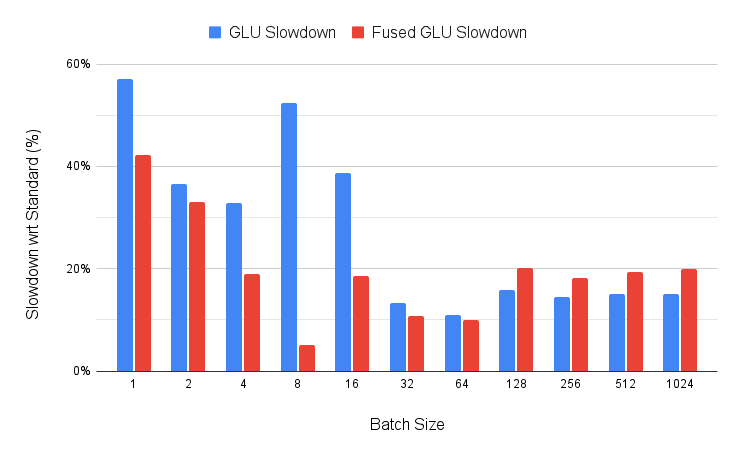
\includegraphics[width=0.8\textwidth]{figures/glu_slowdowns.png}
    \caption{Slowdown of different implementations of Gated Linear Unit. This slowdown is with respect to standard feedforward transformer block. The number of parameters between standard feedforward transformer block and the two GLU implementations are the same.}
    \label{fig:glu-slowdown}
\end{figure}


\section{Limitations and Broader Impact}

\subsection{Limitations}
While we trained two different model sizes, we have not pretrained a MosaicBERT model in the $>1$B parameter range. In this regime, it is possible there will be training stability issues; this is an area of future work.

We also only trained models for 70,000 steps and 178,000 steps of batch size 4096. It is possible that some of the Pareto properties change in the longer regime, although we suspect that this is unlikely.

\subsection{Broader Impact}

BERT models are highly used for NLP tasks. By open-sourcing this work, we hope that our code and models will be used by the wider research community. We recognize however that models like BERT and MosaicBERT are tools that can be used for nefarious purposes, and that biases inherent in the training data can be reflected in the final model artefacts. 

% \newpage
% \newpage

% %\textbf{Extra/Miscellaneous}



% \section{Curve Fitting the Pareto Frontier}
% We can 

% \begin{equation}
%     wct = \Bigg( \Big[-\log\Big(\frac{y - c_1}{-c_2}\Big)\Big]^{-c_4} \Bigg) /c_3
% \end{equation}

% % Alternatively c1 - c2 * np.exp(-(1.0 * c3 * t)**c4)

% \section{BERT vs. RoBERTa}
% RoBERTa finetuning details:
% "We consider a limited hyperparameter
% sweep for each task, with batch sizes ∈ {16, 32}
% and learning rates ∈ {1e−5, 2e−5, 3e−5}, with a
% linear warmup for the first 6% of steps followed by
% a linear decay to 0. We finetune for 10 epochs and
% perform early stopping based on each task’s eval-
% uation metric on the dev set. The rest of the hyper-
% parameters remain the same as during pretraining.
% In this setting, we report the median development
% set results for each task over five random initial-
% izations, without model ensembling."

% "For RTE, STS and MRPC
% we found it helpful to finetune starting from the
% MNLI single-task model, rather than the baseline
% pretrained RoBERTa. W"






% \textbf{TO DO}
% \begin{itemize}
%     \item original BERT training run is an outlier Sellam 2022
%     \item Discuss ELECTRA
%     \item Discuss RoBERTa (trained for much longer), DeBERTa
%     \item Mention how pretraining accuracy is not necessarily correlated with best GLUE score \citep{liu2022same}
% \end{itemize}


% \textbf{TODO: expand discussion here about custom tokenizers. Not sure if this is needed here}
% You can use your own custom vocabulary and tokenizer for your specific domain. A tokenizer splits text into individual “chunks” to be processed by the NLP model. The size and quality of the tokenized vocabulary directly affect both training efficiency and model accuracy. 
% For example, the drug “acetyltransferase” is tokenized by the standard BERT tokenizer into the seven tokens ace, \#\#ty, \#\#lt, \#\#ran, \#\#sf, \#\#eras, \#\#e instead of one or two tokens reflecting the structure and meaning of the term in a biological context [Gu et al. 2020]\todo{cite}. 
% Not only is this tokenization inefficient, but it leads to a suboptimal embedding for biology-related texts that cannot generalize to other related words that incorporate “acetyl” (such as acetylcholine) or “transferase” (such as methyltransferase). 
% Another application of custom tokenization is mathematics, where poor tokenization of numbers (e.g., tokenizing “2023” into the tokens 20 and 23) may limit arithmetic reasoning in language models [Wallace et al. 2019]\todo{cite}. 
% By pretraining your own BERT, you can customize the tokenizer to suit your domain and task.

% Excited about the potential for long sequence lengths

% \textbf{To Do: } discuss question of single epoch vs. multi-epoch \citep{komatsuzaki2019one}


% \subsection{Limitations}

% \textbf{TO DO:} more here

% \begin{itemize}
%     \item We don't compare tokenizers
%     \item We don't go beyond 430M parameters. Stable, rapid pretraining of encoder models larger than 1B parameters is a source for future work
% \end{itemize}


%  Decoupled AdamW with $\beta_1=0.9$ and $\beta_2=0.98$ , and a weight decay value of 1.0e-5. The learning rate schedule begins with a warmup to a maximum learning rate of 5.0e-4 followed by a linear decay to zero. Warmup lasted for 6\% of the full training duration. 

